\documentclass[11pt]{article}
\usepackage[a4paper,textwidth=126mm,textheight=195mm,centering]{geometry}
\usepackage{amsmath,amssymb,booktabs,graphicx,microtype,float,array}
\usepackage[hidelinks]{hyperref}
\usepackage[font=small,labelfont=bf]{caption}
\setlength{\parindent}{1em}
\setlength{\parskip}{0pt}
\title{When does a spectral prior help graph learning? Connectivity-loss estimation under road-network disruptions}
\author{Van-Truong Le\\
\small Faculty of Information Technology, University of Science,\\
\small Viet Nam National University Ho Chi Minh City, Viet Nam\\
\small \href{mailto:23120181@student.hcmus.edu.vn}{23120181@student.hcmus.edu.vn};
\href{mailto:lvtruong@selab.hcmus.edu.vn}{lvtruong@selab.hcmus.edu.vn}\\
\small ORCID: \href{https://orcid.org/0009-0008-7015-7392}{0009-0008-7015-7392}}
\date{}

\begin{document}
\maketitle

\begin{abstract}
Rapid evaluation of many simultaneous road-link disruptions requires a useful
compromise between exact spectral recomputation and local approximation. We
estimate the relative loss of algebraic connectivity after multi-edge deletion
using graph neural networks (GNNs) that learn a bounded correction to a
first-order Fiedler sensitivity. The design is tested under independent and
spatially clustered failures, with graph-disjoint synthetic splits, zero-shot
transfer to five OpenStreetMap (OSM) networks, and geographically blocked
leave-one-area-out transfer. GCN and GraphSAGE backbones, feature ablations, and
analytical or set-based baselines isolate the contribution of the residual
prior, Fiedler node feature, coordinates, and message passing. All uncertainty is calculated from
five seed-level replicates rather than treating correlated scenarios as
independent. In synthetic-to-OSM zero-shot tests, residual learning reduces mean
absolute error relative to a direct GCN by 0.0085 (95\% seed-bootstrap interval
0.0039--0.0131) for independent failures and 0.0121 (0.0026--0.0247) for spatial
failures. However, when models are trained on three OSM areas and tested on a
held-out fourth, the direct GCN is more stable: its errors are 0.135 and 0.109,
compared with 0.161 and 0.144 for the residual model. A reliability-context
extension likewise improves synthetic performance but degrades OSM transfer.
Controlled sparse-eigensolver scaling extends to 20,000 nodes and separates one-time
spectral setup, amortized cost, and update-only cost. These results identify the
spectral residual as a useful but domain-sensitive inductive bias, and delimit
its applicability to structural connectivity rather than hazard or traffic-flow
prediction. Code and cached networks are available at
\href{https://github.com/lee-vtruong/ResiliRoad}{github.com/lee-vtruong/ResiliRoad}.
\end{abstract}

\noindent\textbf{Keywords:} algebraic connectivity; Fiedler vector; graph neural
network; spatial network; infrastructure robustness; domain shift.

\section{Introduction}
Road networks are spatially embedded complex networks whose link losses can
fragment access routes and alter system-wide connectivity. Exhaustive exact
evaluation becomes costly when a planner must screen many multi-link scenarios.
Conversely, a first-order perturbation is fast and interpretable, but its local
linearity can fail under finite deletions, eigenvalue crossings, and
disconnection. This tension motivates a hybrid estimator: retain the known
spectral direction and learn only its nonlinear error.

Algebraic connectivity, the second-smallest Laplacian eigenvalue, is a global
structural quantity~\cite{fiedler1973,mohar1991}. It does not measure travel
demand, congestion, capacity, or recovery. The narrower goal here is fast
structural stress testing: given an intact weighted graph and a set of removed
edges, estimate its relative algebraic-connectivity loss. This distinction is
important because transport robustness has also been defined using system travel
time, capacity loss, accessibility, and repair trajectories
~\cite{scott2006,sullivan2010,sohouenou2021repair}.

This study asks four questions. \textbf{RQ1}: Does learning a residual over a
Fiedler approximation improve direct graph regression? \textbf{RQ2}: Does this
advantage persist under correlated disruptions and geographic domain shift?
\textbf{RQ3}: Which gains come from the explicit prior, Fiedler node feature,
coordinates, or adjacency-aware message passing? \textbf{RQ4}: Where does the
estimator fail and how does its runtime scale?

Rather than asking whether one new GNN architecture wins, the central thesis is
\emph{when a mathematically informed spectral prior helps graph learning under
distribution shift, and when it becomes a biased anchor}. The contributions
are: (i) a bounded residual spectral construction for simultaneous edge
deletions; (ii) controlled feature, GCN/GraphSAGE, and reliability-context
ablations; (iii) two disruption processes on five cached OSM networks; (iv) both
synthetic-to-real zero-shot and geographically disjoint OSM transfer; (v)
seed-paired bootstrap inference, calibration and failure-regime diagnostics; and
(vi) a benchmark separating eigensolver setup, amortized spectral evaluation,
and update-only cost. Importantly, the transfer experiments reveal a limitation:
the residual prior is not uniformly superior once OSM training data are
available.

\section{Related work}
\subsection{Spectral robustness of complex networks}
Fiedler introduced algebraic connectivity as a graph invariant
~\cite{fiedler1973}; later work related Laplacian spectra to expansion,
connectivity, synchronization, and robustness
~\cite{mohar1991,chung1997,jamakovic2008}. Capacity-weighted spectral analysis
has also been used to diagnose transport-network vulnerability~\cite{bell2017}.
For a simple eigenvalue, the squared difference of Fiedler coordinates across an
edge gives the derivative with respect to its weight~\cite{kato1995}. Such derivatives explain
infinitesimal sensitivity, whereas the present task includes several finite edge
deletions. The residual model specifically targets the missing interaction and
higher-order terms rather than replacing spectral analysis.

\subsection{Road-network disruption}
Road robustness depends on graph representation and disruption process.
Multi-granularity analyses of empirical city networks show that structural
conclusions can change with representation~\cite{duan2014}. Link-based indices
using flow or capacity address functional effects~\cite{scott2006,sullivan2010},
while critical-scenario optimization searches for damaging link combinations
~\cite{bagloee2017}. Hazard-independent studies compare random, localized, and
targeted multi-link failures~\cite{sohouenou2021}; temporal analysis of Zurich
also demonstrates process-dependent robustness~\cite{casali2020}. Random road
graph models enable controlled topology experiments~\cite{sohouenou2020}.
Our spatial-cluster mechanism belongs to this stress-testing tradition but is a
geometric proxy, not an empirical hazard model.

Recent evidence makes scale and task definition especially important. Jana et
al.~\cite{jana2023} use an edge-based GNN to rank critical road segments after
disruption, directly motivating learning-based rapid screening; their output is
an edge ranking, whereas ours is a graph-level spectral-loss estimate. Boeing
and Ha~\cite{boeingha2024} simulate 2.4 billion trips across more than 8,000
urban areas in 178 countries, establishing an empirical scale far beyond our
five local networks. Zang et al.~\cite{zang2024} predict dynamic traffic
resilience under rainfall with a multi-granularity GNN; their functional,
temporal target is complementary to our static structural target. Reviews
distinguish connectivity, robustness, vulnerability, and recovery-based
resilience and warn against treating them as synonyms
~\cite{rivera2022,mattsson2015,zeleke2026}.

\subsection{Graph learning and analytical priors}
GCNs aggregate local neighbourhood information and are permutation equivariant
at node level~\cite{kipf2017}. GraphSAGE supplies an inductive aggregation
backbone~\cite{hamilton2017}; GIN studies the expressive limits of neighbourhood
aggregation~\cite{xu2019}, while attention and message-passing frameworks expose
alternative node/edge interactions~\cite{velickovic2018,gilmer2017}. Deep Sets provides an invariant alternative that
does not propagate along edges~\cite{zaheer2017}. Graph Networks have also been
used as learnable physical simulators~\cite{sanchezgonzalez2018}, illustrating
how known structure and learned corrections can coexist. The novelty claimed
here is not the first use of GNNs, residual learning, or spectral metrics. It is
the leakage-resistant empirical separation of an explicit spectral prior from a
spectral node feature, followed by geographic transfer and negative-ablation
analysis on spatial infrastructure networks. Edge-aware modelling is especially
relevant because disruption acts on links: Jana et al.~\cite{jana2023} encode a
road line graph for edge ranking, and Almeida et al.~\cite{almeida2025} report
edge-aware attention for backbone-network load prediction. The present study
instead asks whether a simple node-message-passing estimator benefits from an
explicit spectral prior across domains. Recent JCN work on urban edge removal
uses diffusive transport~\cite{bowater2026}, situating algebraic connectivity
among several legitimate network-function proxies.

\section{Problem formulation and method}
Let $G=(V,E,w)$ be a connected undirected weighted graph, with combinatorial
Laplacian $L=D-A$ and eigenvalues
$0=\lambda_1\leq\lambda_2\leq\cdots$. For disrupted edges $S\subseteq E$, the
target is
\begin{equation}
y(G,S)=\operatorname{clip}\!\left(1-\frac{\lambda_2(G-S)}{\lambda_2(G)},0,1\right).
\label{eq:target}
\end{equation}
Thus a disconnected damaged graph has $y=1$. If $u_2$ is a unit Fiedler vector
and $\lambda_2$ is simple, edge sensitivity is
\begin{equation}
\frac{\partial\lambda_2}{\partial w_{ij}}=(u_{2,i}-u_{2,j})^2.
\end{equation}
The analytical prediction sums intact-graph derivatives:
\begin{equation}
\widehat y_{\mathrm{spec}}=\operatorname{clip}\!\left(
\frac{\sum_{(i,j)\in S}w_{ij}(u_{2,i}-u_{2,j})^2}{\lambda_2(G)},0,1\right).
\label{eq:prior}
\end{equation}

Each damaged graph supplies normalized adjacency and node features: intact
degree, failed-edge incidence, absolute normalized Fiedler coordinate, and two
normalized coordinates. Three 48-unit GCN layers feed mean--max graph pooling
and a two-layer head. The direct model predicts $y$; the residual model predicts
\begin{equation}
\widehat y_{\mathrm{res}}=\operatorname{clip}\left(
\widehat y_{\mathrm{spec}}+\tanh r_\theta(G,S),0,1\right).
\label{eq:residual}
\end{equation}
The bounded correction concentrates capacity on finite-deletion error but can
also inherit domain-specific bias from the prior.

\begin{figure}[H]
\centering
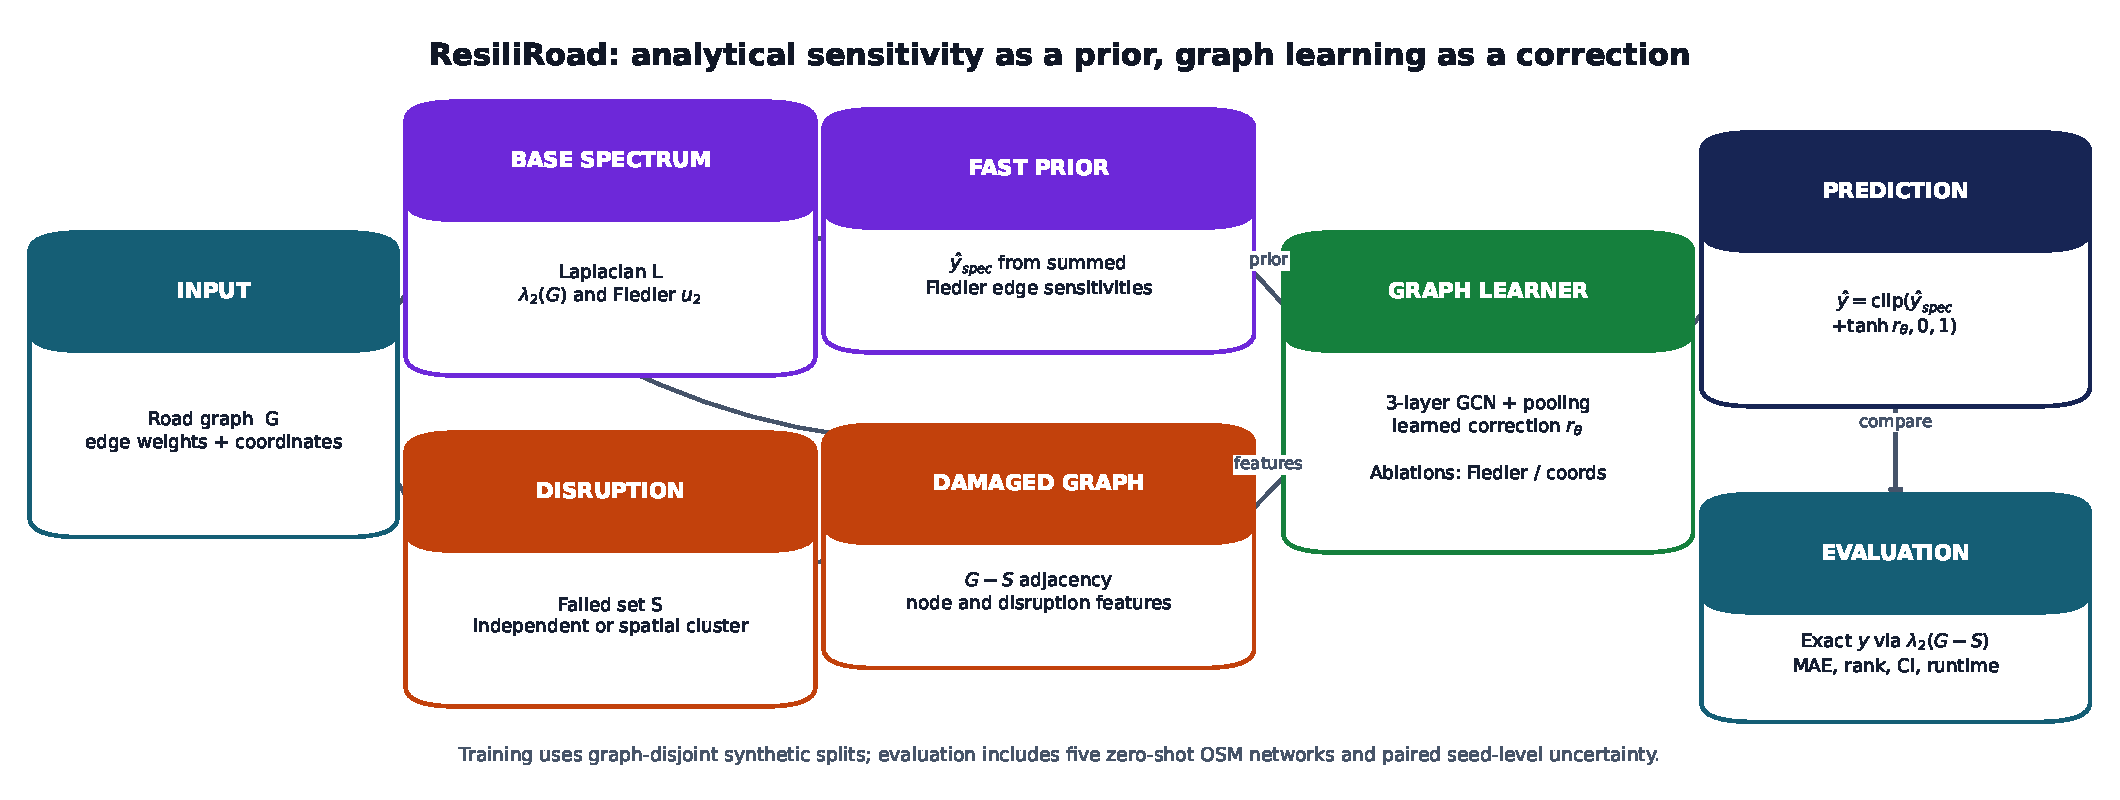
\includegraphics[width=\textwidth]{../figures/method_overview.pdf}
\caption{ResiliRoad workflow. Exact damaged-graph eigendecomposition constructs
labels only. The intact Fiedler vector produces both an optional node feature
and the explicit first-order prior; the GCN learns a bounded correction.}
\label{fig:method}
\par\small\textit{Alt text: A flow diagram splits an intact road graph into an
exact-label branch and a fast spectral-prior branch. Damaged adjacency and node
features enter a GCN whose residual is added to the spectral estimate.}
\end{figure}

The ablation matrix contains direct and residual GCNs with all features, without
Fiedler, and without coordinates; Deep Sets and a summary-statistic MLP are
non-GCN baselines. A further reliability-context residual appends the prior,
normalized failure count, density, and graph size to the prediction head. It
does not use damaged connectivity or any label-derived flag. As a stronger
architecture control, GraphSAGE concatenates each node state with a normalized
neighbourhood aggregate before each of three learned transformations. Its direct
and residual variants use the same features, pooling, optimizer, split, and
stopping rule as the GCN.

\section{Experimental design}
\subsection{Synthetic graphs and disruption processes}
Connected random geometric graphs contain 35--65 nodes and inverse-length edge
conductance. Per seed, 800 scenarios are generated for each failure mode and
entire base-graph families are assigned to train, validation, or test. Each
scenario removes one to eight edges. Independent failure samples edges uniformly.
Spatial-cluster failure chooses a random epicentre and removes the required
number of edges with nearest geometric midpoints. Both modes share the same
failure-count distribution.

\subsection{OpenStreetMap networks}
OSMnx~\cite{boeing2017} was used to obtain 650-m drivable networks around five
Vietnamese sites. Directed multigraphs were simplified, converted to undirected
simple graphs, and restricted to the largest connected component. Conductance
is $100/\mathrm{length}_{\mathrm m}$. Cached GraphML freezes the exact instances
because live OSM data evolve.

\begin{table}[H]
\centering
\caption{OpenStreetMap networks used in the study.}
\label{tab:osm}
\begin{tabular}{lrrr}
\toprule Site & Nodes & Edges & Density\\ \midrule
HCMUS, Ho Chi Minh City&163&221&0.0167\\
VIASM, Hanoi&206&301&0.0143\\
Da Nang&142&203&0.0203\\
Can Tho&114&178&0.0276\\
Da Lat&48&55&0.0488\\ \bottomrule
\end{tabular}
\end{table}

\begin{figure}[H]
\centering
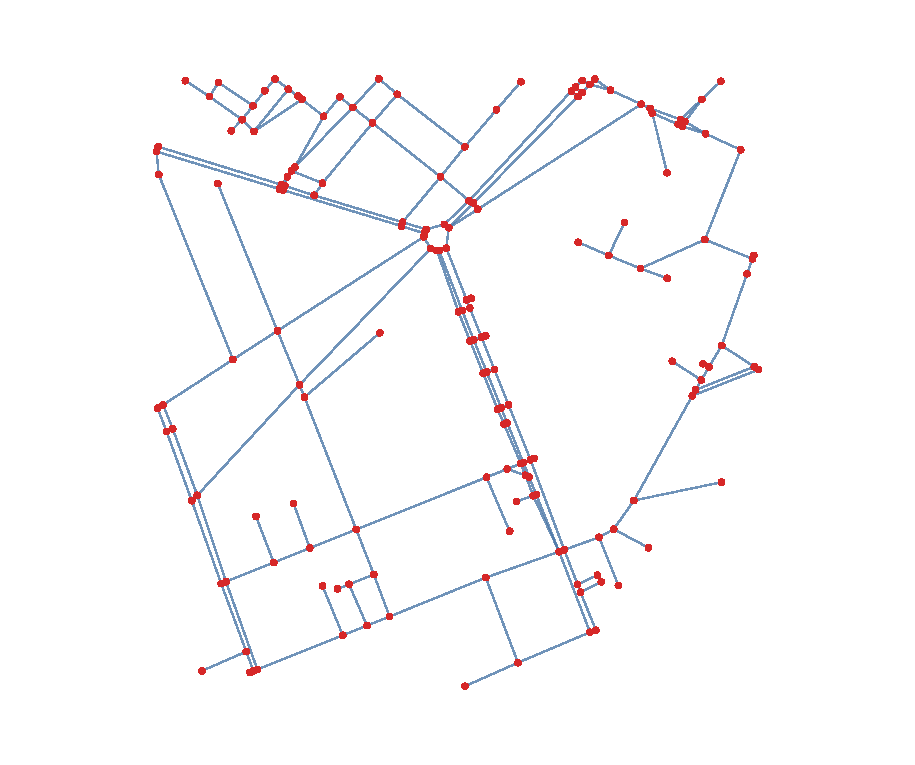
\includegraphics[height=.30\textheight,trim=110 15 110 50,clip]{../outputs/extended_summary/osm_network.pdf}
\caption{Processed HCMUS base network (163 nodes, 221 edges). Disruption
scenarios remove subsets of the displayed links. Map data copyright
OpenStreetMap contributors.}
\label{fig:osm}
\par\small\textit{Alt text: A sparse, irregular street graph is drawn with red
intersection nodes and pale-blue road edges; a dense central corridor connects
several branching neighbourhoods.}
\end{figure}

Two transfer protocols answer different questions. In \emph{zero-shot OSM}, all
learned models train only on synthetic graphs and test on 100 scenarios per
site, mode, and seed. In \emph{leave-one-area-out OSM}, one site is test, the
next site in a fixed rotation is validation, and the remaining three sites are
training. Forty scenarios per site and mode are generated for each of five
seeds; the direct and residual GCNs train for at most 25 epochs. No base area is
shared across train, validation, and test in a fold.

\subsection{Statistics, calibration, and runtime}
Seeds 11, 22, 33, 44, and 55 are independent analysis units. MAE, RMSE,
$R^2$, and Spearman correlation are first computed within seed. Confidence
intervals resample the five seed-level statistics 10,000 times; comparisons
bootstrap within-seed paired differences. No scenario-level $p$-value is used.
Continuous calibration is summarized by regressing target on prediction within
each seed, reporting slope, intercept, and signed mean error. Error slices by
connectivity, failure count, density/site, and spectral clipping are diagnostic.

The original OSM benchmark uses dense symmetric eigendecomposition and
one-scenario neural inference on CPU. A separate controlled benchmark uses
sparse symmetric eigensolves on random geometric graphs with 50--800 nodes. It
reports exact damaged-graph solution, update-only Fiedler sensitivity, and
amortized spectral cost (one intact setup spread over ten scenarios). These
denser graphs are computational stress tests rather than road-realistic samples.

\section{Results}
\subsection{Graph-disjoint synthetic and zero-shot OSM results}
\begin{table}[H]
\centering\small
\caption{MAE as seed mean [95\% seed-bootstrap interval].}
\label{tab:primary}
\resizebox{\textwidth}{!}{%
\begin{tabular}{lcc|cc}
\toprule &\multicolumn{2}{c|}{Synthetic}&\multicolumn{2}{c}{Zero-shot OSM}\\
Method&Independent&Spatial&Independent&Spatial\\ \midrule
Spectral&.069 [.048,.095]&.144 [.102,.183]&.502 [.482,.521]&.650 [.643,.657]\\
Summary MLP&.065 [.051,.079]&.108 [.082,.135]&.281 [.240,.320]&.347 [.269,.425]\\
Deep Sets&.068 [.058,.078]&.105 [.085,.126]&.114 [.105,.123]&.143 [.122,.164]\\
Direct GCN&.077 [.055,.098]&.081 [.067,.097]&.106 [.100,.112]&.102 [.077,.148]\\
Residual GCN&\textbf{.052 [.036,.070]}&\textbf{.065 [.049,.079]}&
\textbf{.097 [.091,.102]}&\textbf{.090 [.071,.124]}\\ \bottomrule
\end{tabular}}
\end{table}

The residual model improves direct-GCN MAE by paired differences 0.0253
[0.0106, 0.0400] and 0.0160 [0.0048, 0.0241] on synthetic independent and
spatial failures. The improvements remain positive in zero-shot OSM: 0.0085
[0.0039, 0.0131] and 0.0121 [0.0026, 0.0247]. Yet the analytical prior alone
has poor OSM calibration despite useful rank information. Removing Fiedler or
coordinates from residual-full yields intervals containing zero; individual
node-feature necessity is therefore not established.

\subsection{Geographically blocked transfer}
\begin{table}[H]
\centering
\caption{Leave-one-area-out OSM performance, seed mean [95\% seed-bootstrap
interval]. Each fold uses three training, one validation, and one test area.}
\label{tab:loao}
\begin{tabular}{lcc}
\toprule Method&Independent MAE&Spatial-cluster MAE\\ \midrule
Direct GCN&\textbf{.135 [.123,.145]}&\textbf{.109 [.106,.112]}\\
Residual GCN&.161 [.118,.216]&.144 [.102,.198]\\ \bottomrule
\end{tabular}
\end{table}

The point-estimate ranking reverses when training is moved into the OSM domain. Direct GCN has
mean $R^2$ 0.714 and 0.747, compared with 0.550 and 0.529 for the residual
model. The paired residual-minus-direct MAE differences are 0.0261
[-0.0122, 0.0824] and 0.0350 [-0.0093, 0.0900]; both intervals include zero,
so five seeds do not establish direct-model superiority. Residual performance is seed-sensitive: independent-failure MAE ranges
from 0.092 to 0.265. Calibration explains part of this instability. Direct-GCN
slopes stay between 0.91 and 1.06; residual slopes fall to 0.58 and 0.69 in the
two poorest seeds, with substantial underprediction. Thus the spectral prior is
helpful under one training distribution but can become a shortcut or a biased
anchor under another.

\subsection{Reliability-context negative ablation}
Adding graph size, density, failure count, and spectral estimate to the residual
head reduces synthetic spatial MAE by 0.0193 [0.0120, 0.0266] and has an
inconclusive $-0.0034$ [-0.0159, 0.0111] change for synthetic independent
failure (negative means improvement). It increases zero-shot OSM spatial MAE by
0.0304 [0.0067, 0.0579]; the independent increase is 0.0452
[-0.0029, 0.1019]. Simple reliability metadata therefore encourages
distribution-specific calibration rather than robust transfer.

\begin{figure}[htbp]
\centering
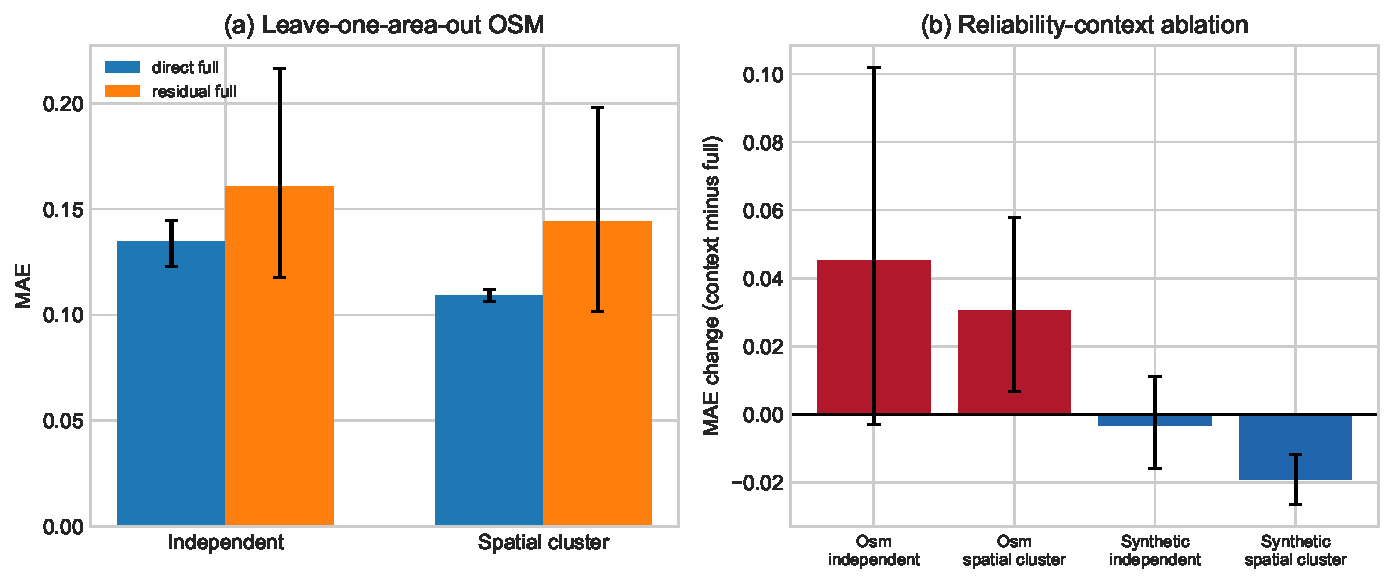
\includegraphics[width=.96\textwidth]{../outputs/journal_summary/transfer_and_ablation.pdf}
\caption{Transfer and negative-ablation results. (a) Leave-one-area-out OSM
MAE. (b) MAE change caused by reliability context; positive values favour
residual-full. Error bars are 95\% seed-bootstrap intervals.}
\label{fig:transfer}
\par\small\textit{Alt text: Two large panels show lower leave-one-area-out
point estimates for direct GCN and reliability context improving synthetic
spatial data but worsening both OSM conditions.}
\end{figure}

\subsection{Backbone robustness}
Replacing GCN propagation with GraphSAGE tests whether the main conclusion is
an artefact of a weak backbone. Table~\ref{tab:backbone} shows that this is not
the case: residual learning improves point-estimate MAE for both backbones in
all four zero-shot conditions. Paired direct-minus-residual differences for
GraphSAGE are 0.0197 [0.0071, 0.0332] and 0.0190 [0.0107, 0.0273] on synthetic
independent and spatial failures, and 0.0069 [0.0032, 0.0096] and 0.0239
[-0.0073, 0.0697] on OSM. The final OSM-spatial interval crosses zero, so the
effect is not declared established there.

\begin{table}[htbp]
\centering
\caption{Architecture control: MAE, seed mean [95\% seed-bootstrap interval].}
\label{tab:backbone}
\resizebox{\textwidth}{!}{\begin{tabular}{llcccc}
\toprule Domain&Failure&Direct GCN&Residual GCN&Direct GraphSAGE&Residual GraphSAGE\\ \midrule
Synthetic&Independent&.077 [.054,.096]&.052 [.036,.071]&.066 [.050,.081]&\textbf{.046 [.034,.063]}\\
Synthetic&Spatial&.081 [.067,.097]&\textbf{.065 [.049,.079]}&.084 [.068,.101]&.065 [.047,.085]\\
OSM&Independent&.106 [.100,.111]&\textbf{.097 [.091,.102]}&.104 [.098,.108]&.097 [.091,.103]\\
OSM&Spatial&.102 [.077,.148]&.090 [.071,.124]&.113 [.082,.164]&\textbf{.089 [.079,.099]}\\ \bottomrule
\end{tabular}}
\end{table}

\subsection{Runtime and error regimes}
On the five small OSM networks, exact dense eigendecomposition averages
5.094 ms per scenario, first-order update 0.018 ms, and residual inference
0.674 ms on CPU. Controlled sparse scaling gives exact times 8.37, 13.41,
14.62, 37.03, and 92.61 ms for 50, 100, 200, 400, and 800 nodes. Update-only
time remains 0.088--0.113 ms; amortized spectral cost is 0.94, 0.89, 1.68,
3.51, and 8.79 ms, while residual-GCN inference is 0.67, 0.70, 0.96, 2.03,
and 5.92 ms. The slight non-monotonicity at small size reflects fixed solver
overhead and graph-to-graph variability; this benchmark is descriptive, not a
complexity proof.

To test the actual screening motivation, a second sparse benchmark uses
connected planar road-like graphs with 1,000, 2,000, 5,000, 10,000, and 20,000
nodes and about 2.1 edges per node. Nodes occupy a normalized, near-square
regular lattice. Horizontal and vertical nearest-neighbour edges form a
connected truncated grid; each eligible cell independently receives its
northwest diagonal with probability 0.12, which preserves planarity. Edge
conductance is inverse Euclidean length. Each timed disruption removes eight
uniformly sampled edges; base-graph connectivity is guaranteed by the grid
backbone. At 20,000 nodes, sparse exact recomputation
requires 1,302.4 ms per damaged graph. Intact eigensolver setup costs 1,335.3
ms once; amortized over 1,000 screened scenarios, the prior costs 1.41 ms,
sparse GNN inference 21.76 ms, and the combined path 23.17 ms. Thus the measured
screening path is 56 times faster at the largest size, conditional on reusing
one intact graph. Only three scenarios on each of two generated graphs are
timed per size, and the large graphs are not used for accuracy training; these
measurements support computational scaling, not predictive generalization.

\begin{figure}[htbp]
\centering
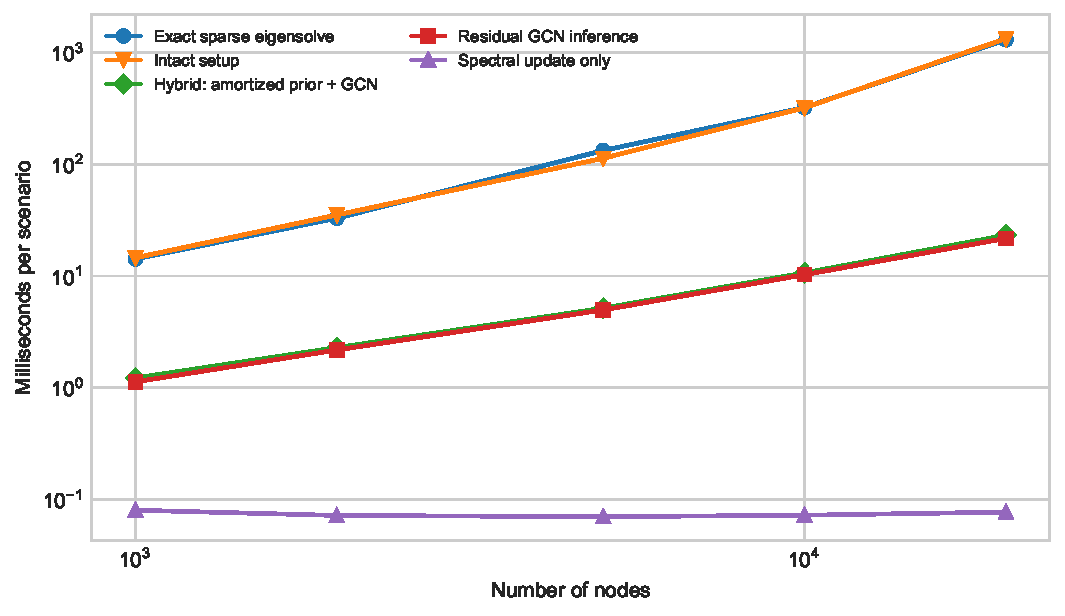
\includegraphics[width=.92\textwidth]{../outputs/journal_summary/large_scale_runtime.pdf}
\caption{Sparse CPU scaling from 1,000 to 20,000 nodes. Exact recomputation is
timed per damaged graph; the hybrid curve combines intact spectral setup
amortized over 1,000 scenarios with first-order evaluation and sparse GNN
inference. Points are means over two graphs and three scenarios per graph.}
\label{fig:scaling}
\par\small\textit{Alt text: A log--log runtime plot shows exact sparse
eigendecomposition rising to about 1.3 seconds at 20,000 nodes, while the
amortized hybrid path rises to about 23 milliseconds.}
\end{figure}

In zero-shot OSM, residual-full MAE is 0.070 for connected damaged graphs and
0.112 after disconnection. Site errors range from 0.041 (Can Tho) to 0.189
(Da Lat). The densest site is also the smallest and hardest, so density cannot
be interpreted causally. No evaluated first-order estimate clips at one; the
requested clipped/unclipped comparison is therefore undefined. The largest
leave-one-area-out errors are retained in a machine-readable table instead of
being removed as outliers.

\section{Discussion}
The central result is a condition, not a new-architecture claim. A spectral
residual improves both GCN and GraphSAGE on graph-disjoint synthetic tests and
usually when transferred zero-shot to OSM. It combines the prior's ranking
signal with learned nonlinear calibration. However, blocked OSM transfer and
reliability-context ablation show that the same inductive bias can amplify
domain-specific error. The prior then behaves as a shortcut or biased anchor:
optimization remains close to a convenient analytical signal even when its
calibration has shifted. Direct prediction is more stable when training already
contains real-road graphs. Consequently, whether a mathematical prior helps is
an empirical distribution-shift question, not an architectural guarantee.

The study also separates the explicit prior from Fiedler node information.
Neither Fiedler nor coordinate removal produces a stable loss, whereas replacing
the residual architecture does. The robust ingredient in the first protocol is
therefore how mathematical and learned estimates are combined, not merely the
presence of an eigenvector channel. The poor Deep Sets ranking in several
regimes supports adjacency-aware propagation, while the summary MLP shows that
coarse graph statistics are insufficient.

\subsection{Limitations}
Five 650-m Vietnamese neighbourhoods do not establish city-scale or
cross-country predictive generality. Their size and density are confounded. The
synthetic geometric generator and large-scaling graphs are controlled proxies,
not metropolitan OSM accuracy datasets. Spatial clusters are not calibrated to flood,
landslide, earthquake, construction, or conflict data. Algebraic connectivity
is structural: it omits direction, demand, congestion, capacity, travel time,
accessibility, and restoration. Only five seed replicates limit precision, and
no probabilistic predictive intervals are produced. Sparse batched neural
implementations and spectral sparsification~\cite{spielman2011} may change
runtime rankings at still larger scale.

Future work should pre-register larger metropolitan regions, use nested blocked
validation across countries, and factor graph size from density. Hazard rasters
could define correlated failures, while traffic assignment could test whether
structural loss predicts service degradation. Mixture-of-experts or learned
gating may decide when to trust the prior; conformal methods could add
graph-population prediction regions. These extensions should preserve area-level
replication rather than inflate sample size with correlated scenarios.

\section{Conclusion}
Residual spectral graph learning offers an interpretable, fast estimator of
finite multi-edge connectivity loss, but its advantage depends on training
domain. The method beats direct GCN and GraphSAGE under graph-disjoint synthetic
and most synthetic-to-OSM zero-shot evaluations; direct GCN is more stable under blocked
OSM-to-OSM transfer. Reporting both outcomes, along with ablations, hierarchical
uncertainty, calibration, error cases, and separated runtime costs, provides a
reproducible account of when a Fiedler prior helps and when it does not.

\section*{Data and code availability}
Code, cached OSM-derived GraphML, manifests, experiment scripts, environment
versions, compact result tables, and release metadata are available as
ResiliRoad version 1.0.0~\cite{resiliroad}.
OSM data are licensed under the Open Data Commons Open Database License and are
attributed to OpenStreetMap contributors~\cite{osm}. Release metadata are
included so that the exact submitted version can be archived and cited
persistently without relying on a mutable development branch.

\section*{Funding}
This research received no external funding.

\section*{Conflict of interest}
The author declares no conflict of interest.

\section*{Acknowledgements and AI-use disclosure}
Generative AI tools were used for language editing and software-development
assistance. The author designed the study, verified the implementation and
results, and takes responsibility for the manuscript.

\appendix
\section{Reproducibility details}
All models use AdamW, mean-squared error, validation early stopping, and one
PyTorch compute thread. Core runs use at most 80 epochs; blocked OSM transfer
uses at most 25. Software versions are Python 3.13.11, NumPy 2.4.4, SciPy
1.17.1, NetworkX 3.6.1, pandas 2.2.3, scikit-learn 1.9.0, PyTorch 2.11.0
(CPU), Matplotlib 3.11.1, OSMnx 2.1.1, and GeoPandas 1.1.4. The machine has 16
logical AMD64 CPUs; CUDA was unavailable. Scripts record exact seeds and emit
scenario predictions, training histories, fold assignments, runtime summaries,
bootstrap tables, calibration diagnostics, and worst cases.
The architecture-control runs use identical data and training settings for GCN
and GraphSAGE. Large-scale runtime graphs use a normalized near-square lattice,
four-neighbour grid backbone, independent northwest diagonals with probability
0.12, and inverse-length conductance; the deterministic grid guarantees a
connected base graph and yields mean degree approximately 4.2. Sparse
\texttt{eigsh} uses a fixed starting vector. The intact setup cost is
reported both separately and amortized over 1,000 scenarios, preventing
preprocessing from being hidden in the speed comparison.

\begin{thebibliography}{99}
\bibitem{fiedler1973} M. Fiedler, Algebraic connectivity of graphs,
\emph{Czechoslovak Mathematical Journal} 23 (1973), 298--305.
\bibitem{mohar1991} B. Mohar, The Laplacian spectrum of graphs, in
\emph{Graph Theory, Combinatorics, and Applications}, Wiley, 1991, 871--898.
\bibitem{chung1997} F.R.K. Chung, \emph{Spectral Graph Theory}, CBMS Regional
Conference Series in Mathematics 92, American Mathematical Society, 1997.
\bibitem{kato1995} T. Kato, \emph{Perturbation Theory for Linear Operators},
Springer, 1995. doi:10.1007/978-3-642-66282-9.
\bibitem{jamakovic2008} A. Jamakovic and P. Van Mieghem, On the robustness of
complex networks by using the algebraic connectivity, \emph{NETWORKING 2008},
LNCS 4982 (2008), 183--194. doi:10.1007/978-3-540-79549-0\_16.
\bibitem{scott2006} D.M. Scott et al., Network robustness index: a new method
for identifying critical links, \emph{Journal of Transport Geography} 14
(2006), 215--227. doi:10.1016/j.jtrangeo.2005.10.003.
\bibitem{sullivan2010} J.L. Sullivan et al., Identifying critical road segments
and measuring system-wide robustness, \emph{Transportation Research A} 44
(2010), 323--336. doi:10.1016/j.tra.2010.02.003.
\bibitem{duan2014} Y. Duan and F. Lu, Robustness of city road networks at
different granularities, \emph{Physica A} 411 (2014), 21--34.
doi:10.1016/j.physa.2014.05.073.
\bibitem{bagloee2017} S.A. Bagloee et al., Identifying critical disruption
scenarios and a global robustness index tailored to real life road networks,
\emph{Transportation Research E} 98 (2017), 60--81.
doi:10.1016/j.tre.2016.12.003.
\bibitem{sohouenou2020} P.Y.R. Sohouenou et al., Using a random road graph
model to understand road networks robustness to link failures,
\emph{International Journal of Critical Infrastructure Protection} 29 (2020),
100353. doi:10.1016/j.ijcip.2020.100353.
\bibitem{casali2020} Y. Casali and H.R. Heinimann, Robustness response of the
Zurich road network under different disruption processes, \emph{Computers,
Environment and Urban Systems} 81 (2020), 101460.
doi:10.1016/j.compenvurbsys.2020.101460.
\bibitem{sohouenou2021} P.Y.R. Sohouenou et al., Using a hazard-independent
approach to understand road-network robustness to multiple disruption scenarios,
\emph{Transportation Research D} 93 (2021), 102672.
doi:10.1016/j.trd.2020.102672.
\bibitem{sohouenou2021repair} P.Y.R. Sohouenou and L.A.C. Neves, Assessing the
effects of link-repair sequences on road network resilience,
\emph{International Journal of Critical Infrastructure Protection} 34 (2021),
100448. doi:10.1016/j.ijcip.2021.100448.
\bibitem{bruneau2003} M. Bruneau et al., A framework to quantitatively assess
and enhance the seismic resilience of communities, \emph{Earthquake Spectra}
19 (2003), 733--752. doi:10.1193/1.1623497.
\bibitem{mattsson2015} L.-G. Mattsson and E. Jenelius, Vulnerability and
resilience of transport systems---a discussion of recent research,
\emph{Transportation Research A} 81 (2015), 16--34.
doi:10.1016/j.tra.2015.06.002.
\bibitem{bell2017} M.G.H. Bell et al., Investigating transport network
vulnerability by capacity weighted spectral analysis, \emph{Transportation
Research B} 99 (2017), 251--266. doi:10.1016/j.trb.2017.03.002.
\bibitem{rivera2022} D.A. Rivera-Royero et al., Road network performance: a
review on relevant concepts, \emph{Computers \& Industrial Engineering} 165
(2022), 107927. doi:10.1016/j.cie.2021.107927.
\bibitem{jana2023} D. Jana, S. Malama, S. Narasimhan and E. Taciroglu,
Edge-based graph neural network for ranking critical road segments in a
network, \emph{PLOS ONE} 18 (2023), e0296045.
doi:10.1371/journal.pone.0296045.
\bibitem{boeingha2024} G. Boeing and P. Ha, Resilient by design: simulating
street network disruptions across every urban area in the world,
\emph{Transportation Research A} 182 (2024), 104016.
doi:10.1016/j.tra.2024.104016.
\bibitem{zang2024} Z. Zang et al., Predictive resilience assessment of road
networks based on dynamic multi-granularity graph neural network,
\emph{Neurocomputing} 601 (2024), 128207.
doi:10.1016/j.neucom.2024.128207.
\bibitem{zeleke2026} A. Zeleke, M. Tira and C. Scaini, Resilience of road
networks to natural hazards: a systematic literature review,
\emph{Transportation Engineering} 23 (2026), 100420.
doi:10.1016/j.treng.2026.100420.
\bibitem{kipf2017} T.N. Kipf and M. Welling, Semi-supervised classification
with graph convolutional networks, \emph{ICLR}, 2017. arXiv:1609.02907.
\bibitem{hamilton2017} W.L. Hamilton, R. Ying and J. Leskovec, Inductive
representation learning on large graphs, \emph{NeurIPS} 30 (2017).
\bibitem{gilmer2017} J. Gilmer et al., Neural message passing for quantum
chemistry, \emph{ICML} 70 (2017), 1263--1272.
\bibitem{velickovic2018} P. Veli\v{c}kovi\'c et al., Graph attention networks,
\emph{ICLR}, 2018.
\bibitem{xu2019} K. Xu et al., How powerful are graph neural networks?,
\emph{ICLR}, 2019. arXiv:1810.00826.
\bibitem{zaheer2017} M. Zaheer et al., Deep Sets, \emph{NeurIPS} 30 (2017).
\bibitem{sanchezgonzalez2018} A. Sanchez-Gonzalez et al., Graph networks as
learnable physics engines for inference and control, \emph{ICML} (2018),
4470--4479.
\bibitem{almeida2025} F. Almeida et al., Leveraging edge-aware graph neural
networks to predict node load in backbone networks, \emph{Journal of Complex
Networks} 13 (2025), cnaf050. doi:10.1093/comnet/cnaf050.
\bibitem{bowater2026} R.J. Bowater, Impact of one-way streets on diffusive
transport, \emph{Journal of Complex Networks} 14 (2026), cnag019.
doi:10.1093/comnet/cnag019.
\bibitem{spielman2011} D.A. Spielman and N. Srivastava, Graph sparsification by
effective resistances, \emph{SIAM Journal on Computing} 40 (2011), 1913--1926.
doi:10.1137/080734029.
\bibitem{boeing2017} G. Boeing, OSMnx: new methods for acquiring, constructing,
analyzing, and visualizing complex street networks, \emph{Computers,
Environment and Urban Systems} 65 (2017), 126--139.
doi:10.1016/j.compenvurbsys.2017.05.004.
\bibitem{osm} OpenStreetMap contributors, OpenStreetMap, 2026,
\url{https://www.openstreetmap.org/copyright}.
\bibitem{resiliroad} V.-T. Le, ResiliRoad: spectral-prior graph learning for
road-network disruption screening, version 1.0.0, 2026,
\url{https://github.com/lee-vtruong/ResiliRoad}.
\end{thebibliography}
\end{document}
